% Options for packages loaded elsewhere
% Options for packages loaded elsewhere
\PassOptionsToPackage{unicode}{hyperref}
\PassOptionsToPackage{hyphens}{url}
\PassOptionsToPackage{dvipsnames,svgnames,x11names}{xcolor}
%
\documentclass[
  12pt]{article}
\usepackage{xcolor}
\usepackage{amsmath,amssymb}
\setcounter{secnumdepth}{5}
\usepackage{iftex}
\ifPDFTeX
  \usepackage[T1]{fontenc}
  \usepackage[utf8]{inputenc}
  \usepackage{textcomp} % provide euro and other symbols
\else % if luatex or xetex
  \usepackage{unicode-math} % this also loads fontspec
  \defaultfontfeatures{Scale=MatchLowercase}
  \defaultfontfeatures[\rmfamily]{Ligatures=TeX,Scale=1}
\fi
\usepackage{lmodern}
\ifPDFTeX\else
  % xetex/luatex font selection
\fi
% Use upquote if available, for straight quotes in verbatim environments
\IfFileExists{upquote.sty}{\usepackage{upquote}}{}
\IfFileExists{microtype.sty}{% use microtype if available
  \usepackage[]{microtype}
  \UseMicrotypeSet[protrusion]{basicmath} % disable protrusion for tt fonts
}{}
\makeatletter
\@ifundefined{KOMAClassName}{% if non-KOMA class
  \IfFileExists{parskip.sty}{%
    \usepackage{parskip}
  }{% else
    \setlength{\parindent}{0pt}
    \setlength{\parskip}{6pt plus 2pt minus 1pt}}
}{% if KOMA class
  \KOMAoptions{parskip=half}}
\makeatother
% Make \paragraph and \subparagraph free-standing
\makeatletter
\ifx\paragraph\undefined\else
  \let\oldparagraph\paragraph
  \renewcommand{\paragraph}{
    \@ifstar
      \xxxParagraphStar
      \xxxParagraphNoStar
  }
  \newcommand{\xxxParagraphStar}[1]{\oldparagraph*{#1}\mbox{}}
  \newcommand{\xxxParagraphNoStar}[1]{\oldparagraph{#1}\mbox{}}
\fi
\ifx\subparagraph\undefined\else
  \let\oldsubparagraph\subparagraph
  \renewcommand{\subparagraph}{
    \@ifstar
      \xxxSubParagraphStar
      \xxxSubParagraphNoStar
  }
  \newcommand{\xxxSubParagraphStar}[1]{\oldsubparagraph*{#1}\mbox{}}
  \newcommand{\xxxSubParagraphNoStar}[1]{\oldsubparagraph{#1}\mbox{}}
\fi
\makeatother


\usepackage{longtable,booktabs,array}
\usepackage{calc} % for calculating minipage widths
% Correct order of tables after \paragraph or \subparagraph
\usepackage{etoolbox}
\makeatletter
\patchcmd\longtable{\par}{\if@noskipsec\mbox{}\fi\par}{}{}
\makeatother
% Allow footnotes in longtable head/foot
\IfFileExists{footnotehyper.sty}{\usepackage{footnotehyper}}{\usepackage{footnote}}
\makesavenoteenv{longtable}
\usepackage{graphicx}
\makeatletter
\newsavebox\pandoc@box
\newcommand*\pandocbounded[1]{% scales image to fit in text height/width
  \sbox\pandoc@box{#1}%
  \Gscale@div\@tempa{\textheight}{\dimexpr\ht\pandoc@box+\dp\pandoc@box\relax}%
  \Gscale@div\@tempb{\linewidth}{\wd\pandoc@box}%
  \ifdim\@tempb\p@<\@tempa\p@\let\@tempa\@tempb\fi% select the smaller of both
  \ifdim\@tempa\p@<\p@\scalebox{\@tempa}{\usebox\pandoc@box}%
  \else\usebox{\pandoc@box}%
  \fi%
}
% Set default figure placement to htbp
\def\fps@figure{htbp}
\makeatother





\setlength{\emergencystretch}{3em} % prevent overfull lines

\providecommand{\tightlist}{%
  \setlength{\itemsep}{0pt}\setlength{\parskip}{0pt}}



 
\usepackage[]{natbib}
\bibliographystyle{agsm}


\addtolength{\oddsidemargin}{-.5in}%
\addtolength{\evensidemargin}{-1in}%
\addtolength{\textwidth}{1in}%
\addtolength{\textheight}{1.7in}%
\addtolength{\topmargin}{-1in}%
\makeatletter
\@ifpackageloaded{caption}{}{\usepackage{caption}}
\AtBeginDocument{%
\ifdefined\contentsname
  \renewcommand*\contentsname{Table of contents}
\else
  \newcommand\contentsname{Table of contents}
\fi
\ifdefined\listfigurename
  \renewcommand*\listfigurename{List of Figures}
\else
  \newcommand\listfigurename{List of Figures}
\fi
\ifdefined\listtablename
  \renewcommand*\listtablename{List of Tables}
\else
  \newcommand\listtablename{List of Tables}
\fi
\ifdefined\figurename
  \renewcommand*\figurename{Figure}
\else
  \newcommand\figurename{Figure}
\fi
\ifdefined\tablename
  \renewcommand*\tablename{Table}
\else
  \newcommand\tablename{Table}
\fi
}
\@ifpackageloaded{float}{}{\usepackage{float}}
\floatstyle{ruled}
\@ifundefined{c@chapter}{\newfloat{codelisting}{h}{lop}}{\newfloat{codelisting}{h}{lop}[chapter]}
\floatname{codelisting}{Listing}
\newcommand*\listoflistings{\listof{codelisting}{List of Listings}}
\makeatother
\makeatletter
\makeatother
\makeatletter
\@ifpackageloaded{caption}{}{\usepackage{caption}}
\@ifpackageloaded{subcaption}{}{\usepackage{subcaption}}
\makeatother
\usepackage{bookmark}
\IfFileExists{xurl.sty}{\usepackage{xurl}}{} % add URL line breaks if available
\urlstyle{same}
\hypersetup{
  pdftitle={Shark Bite Survivorship of Northern Elephant Seals (Mirounga angustirostris)},
  pdfauthor={Nat Bilal; Sharry Eydel},
  colorlinks=true,
  linkcolor={blue},
  filecolor={Maroon},
  citecolor={Blue},
  urlcolor={Blue},
  pdfcreator={LaTeX via pandoc}}



\begin{document}


\def\spacingset#1{\renewcommand{\baselinestretch}%
{#1}\small\normalsize} \spacingset{1}


%%%%%%%%%%%%%%%%%%%%%%%%%%%%%%%%%%%%%%%%%%%%%%%%%%%%%%%%%%%%%%%%%%%%%%%%%%%%%%

\date{December 9, 2025}
\title{\bf Shark Bite Survivorship of Northern Elephant Seals (Mirounga
angustirostris)}
\author{
Nat Bilal\thanks{The authors gratefully acknowledge Doctor Marcela
Alfaro Córdoba from UC Santa Cruz for providing the mapping code for our
analyses.}\\
Department of Ecology and Evolutionary Biology, University of
California, Santa Cruz\\
and\\Sharry Eydel\\
Department of Engineering, University of California, Santa Cruz\\
}
\maketitle

\bigskip
\bigskip
\begin{abstract}

\end{abstract}


\newpage
\spacingset{1.9} % DON'T change the spacing!


\section{Introduction}\label{sec-intro}

Northern elephant seals are a seasonal resident of Año Nuevo State Park
in San Mateo County, California. This species is a keystone species,
serving as an indicator of its marine environments, and researchers'
observations of the animals on land can often point to individuals'
experiences at sea (\citet{beltran2025}). The goal of this project is to
perform exploratory data analysis on key variables relating to the
prevalence and survivorship of shark bites on the Año Nuevo colony of
elephant seals. By learning more about the predator-prey dynamics these
animals experience, scientists hope to understand more about the several
marine ecosystems in which they exist (\citet{andrzejaczek2022}). For
our research questions, we will focus on the following:

\begin{enumerate}
\def\labelenumi{\arabic{enumi}.}
\item
  How do rates of shark bites differ between sex and age classes?
\item
  Do sex and/or age predict the likelihood of a shark bite's location on
  the body?
\item
  In which areas of the colony do shark-bitten elephant seals appear
  more frequently?
\end{enumerate}

Our dataset is subsetted from privately available data from the ongoing
population monitoring effort of Año Nuevo State Park between the years
of 1979 and 2024. This dataset, selected from observations indicating
the presence of a shark bite on an observed seal, contains 225
observations with 106 unique seals. Therefore, the dataset and research
questions outlined above are limited by the survivorship bias exhibited
by seals who survived their trip to land and were observed at the Año
Nuevo colony. For our research questions, we focused on the following
categorical variables from the greater dataset as detailed below:

\begin{itemize}
\tightlist
\item
  animalID: a four- to five-digit numeric identifier unique to a seal,
  assigned upon first observation,
\item
  regionID: areas numbered one through nineteen representing locations
  throughout the park where the seal was observed, simplified from
  colony map locations,~
\item
  age class: a seal's observed age recoded as binary, either adult
  (``ad'') or juvenile (``juv''),
\item
  sex: a seal's observed sex, either male (M) or female (F), and~
\item
  bite location: where on the seal's body a bite was observed,
  three-level: head or neck (``end''), body (``body''), or flippers
  (``flip''), coded from string comments.
\end{itemize}

\section{Exploratory Data Analysis}\label{exploratory-data-analysis}

Data cleaning mainly consisted of recoding string entries into
categories and/or new variables and removing any irrelevant cases (i.e.,
observations from different colonies or of seals with non-predatory,
``cookie cutter shark'' bites). Of the columns we used for our analysis,
43 out of the 180 rows remaining after cleaning had at least one missing
value, which we did not alter for analyses. The aforementioned variables
are summarized below.~

The graph below displays the top 10 most frequently observed seals in
the dataset, with animalID 41117 being the most observed at 27
observations (Figure 1). To account for multiple potential observations
per seal, the dataset was sorted by animalID and only the most recent
observation for each seal was retained for analyses.~

\begin{figure}

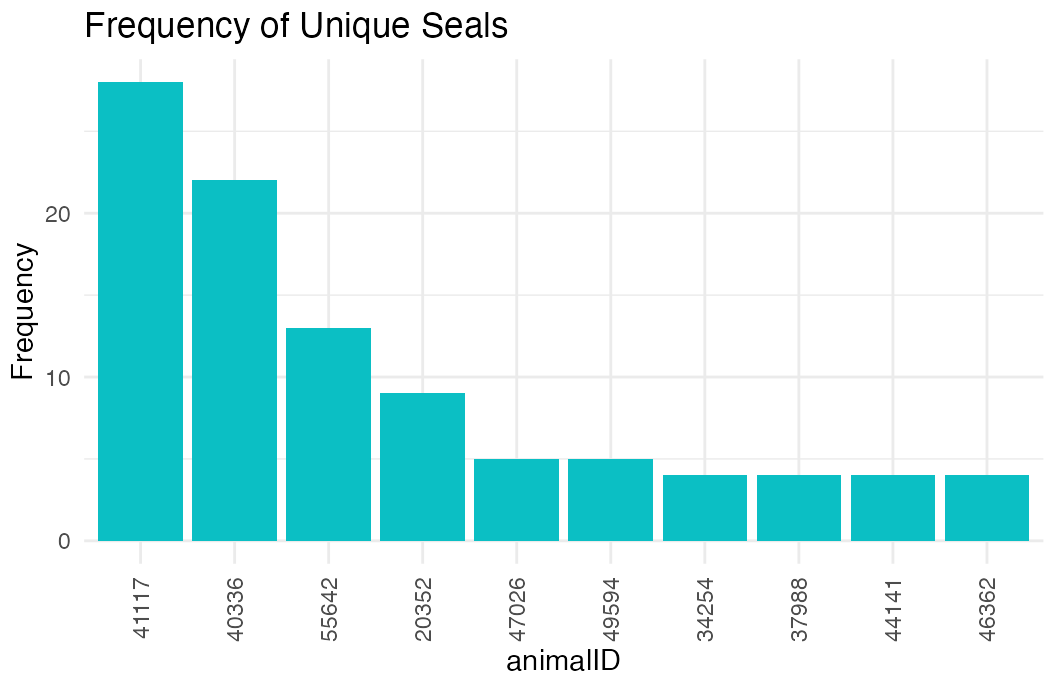
\includegraphics[width=5in,height=\textheight,keepaspectratio]{animalID_graph.png}

\caption{\label{fig-one}Most frequently observed seals.}

\end{figure}%

In the bar plot below, counts of seals per regionID are colored by
whether their location was on the beach or inland, with missing data on
location for 13 seals (Figure 2). The numbers indicated for regionID
correlate with those on the accompanying map (Figure 3). Based on this
plot, we can see that a majority of seals were sighted around the middle
of the colony between and including sites 4 to 11, with the beach
locations being the most frequented.

\begin{figure}

\centering{

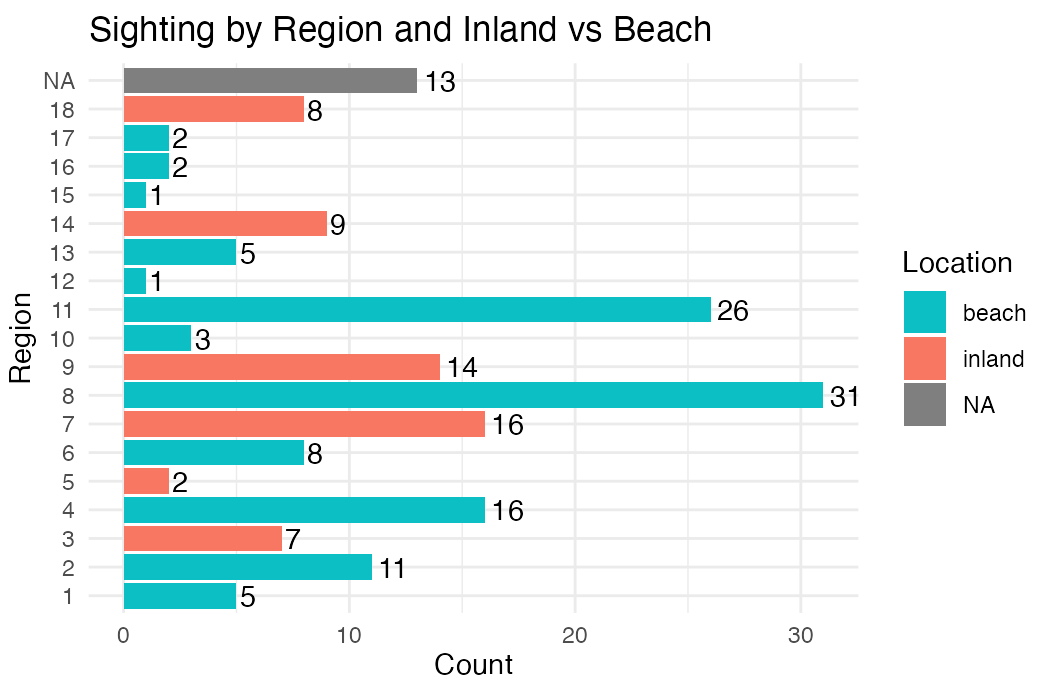
\includegraphics[width=4.59375in,height=\textheight,keepaspectratio]{regionID_graph.png}

}

\caption{\label{fig-two}Frequency of observations by region as numbered
on corresponding map. Sightings are most frequent at sites 4 through 11,
the middle of the colony.}

\end{figure}%

\begin{figure}

\centering{

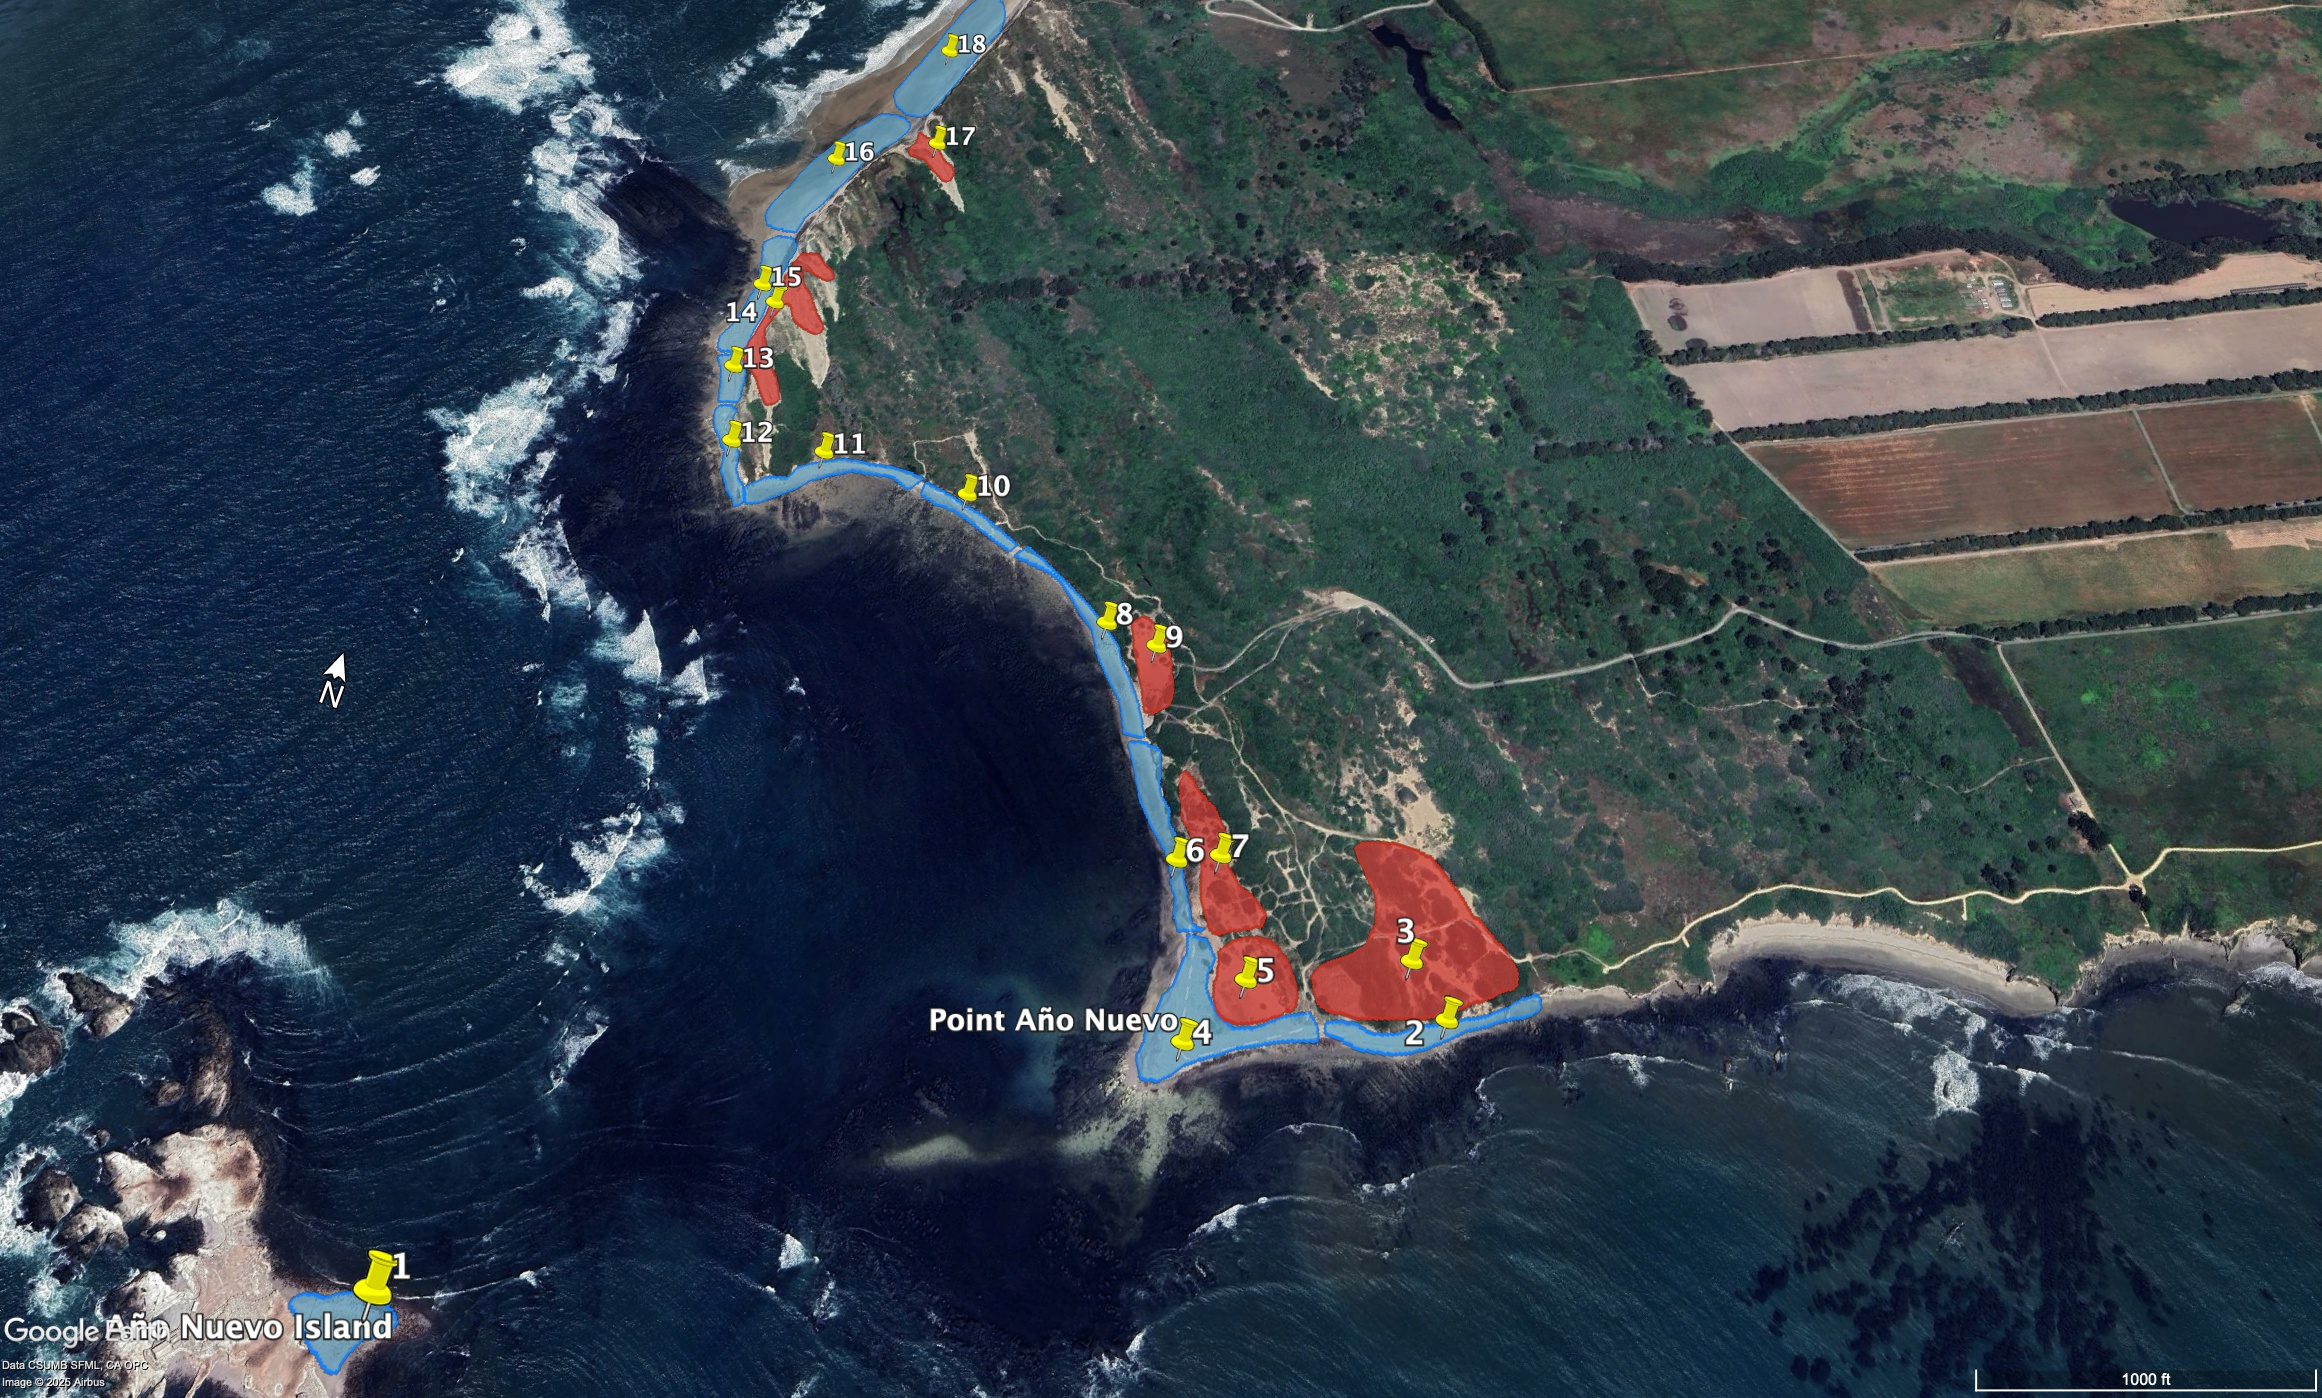
\includegraphics[width=3.5in,height=\textheight,keepaspectratio]{AreaCleanInlandBeach.jpg}

}

\caption{\label{fig-three}Año Nuevo State Park northern elephant seal
colony divided by regionID locations derived from grouped map locations
on the original population monitoring map. regionID locations are
denoted with yellow pushpins and their corresponding number. Inland
locations are colored red, and beach locations are colored light blue.}

\end{figure}%

The next bar plot shows the frequency of each bite location per a seal's
sex (Figure 4). As depicted, females appear to receive bites on their
body most frequently, disproportionately more so than males or seals
whose sex was not recorded.

\begin{figure}

\centering{

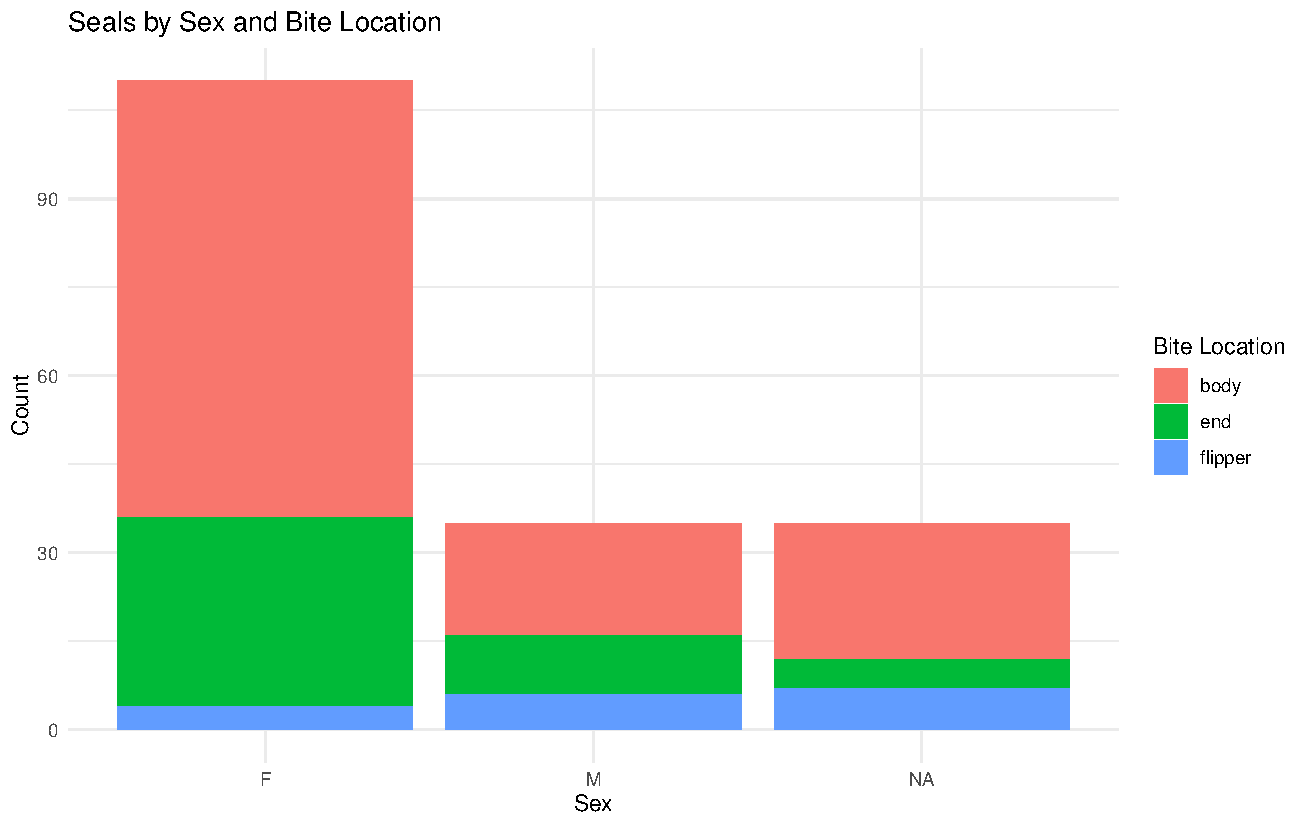
\includegraphics[width=4.75in,height=\textheight,keepaspectratio]{Seals_Sex_BiteLoc.pdf}

}

\caption{\label{fig-four}Shark bite locations on observed seals' bodies.
Bites on the body are disproportionately more frequent among female
seals.}

\end{figure}%

The following table displays contingencies of sex and age class status
to characterize individuals in the dataset. The most common category of
observed seals are adult females. The sample sizes within groupings
indicate insufficient counts for a Chi-square test of independence.

\begin{longtable}[]{@{}lll@{}}
\caption{Contingencies of Sex by Age
class.}\label{tbl-one}\tabularnewline
\toprule\noalign{}
& Adult & Juvenile \\
\midrule\noalign{}
\endfirsthead
\toprule\noalign{}
& Adult & Juvenile \\
\midrule\noalign{}
\endhead
\bottomrule\noalign{}
\endlastfoot
Female & 23 & 2 \\
Male & 5 & 19 \\
\end{longtable}

Overall, the data appear unevenly distributed, with a far smaller number
of unique seal observations than previously expected based on the size
of the dataset. This finding indicates that analyses requiring high
statistical power may not be appropriate for these data.

\section{Methods}\label{sec-meth}

\textbf{Bite Demographics}

To explore how rates of shark bites differ between sex and age classes,
we used Fisher's Exact Test, as it is the most appropriate method when
frequency groupings differ disproportionately or are exceptionally
small. We completed this analysis using the base R command
\emph{fisher.test().} ~~

\textbf{Bite Body Location}

To determine whether bites on certain areas of the body were more likely
for certain demographic groups of seals, we fitted three separate
logistic regression models for each location on the body (end, body, and
flippers). By creating binary variables for each bite location (presence
indicated by 1, absence indicated by 0), we were able to create
regression models fitting age and sex as predictors of each bite
location with an interaction term between the two predictors: \[
logit = log(\frac{p}{1-p}) = \beta_0 + \beta_1X_1 + \beta_2X_2 + \beta_3X_1X_2
\]

Assumptions were assessed using built-in functions in R, and analyses
were performed in base R using the function \emph{glm().} Graphs were
computed using ggplot2 (\citet{patil2021}).

\textbf{Bite Geographic Location}

Lastly, to explore the frequency of shark-bitten seals by location, we
used the \emph{sf} package (\citet{pebesma2018}) to visualize counts on
a georeferenced map of the park. As the purpose of this visualization
was exploratory, graphing frequencies alone without analyzing
significant differences was appropriate. To do this, we derived
coordinate points from the average center of each regionID using
GoogleEarthPro. These coordinates were transferred into a csv file,
imported into R, and transformed into a simple feature object. Our
reference map was sourced from the San Mateo County GIS imagery database
and specified to just the area of the colony. This map was also imported
and transformed into a shape file before graphing frequencies of
observations by regionID coordinate, with point size indicating
observation frequency. This final map was graphed using ggplot2.

\section{Results}\label{sec-verify}

\textbf{Fisher's Exact Test}

Counts between groupings were significantly different (\emph{p}
\textless{} .001), with adults more likely to be female and juveniles
more likely to be male (Figure 5).

\begin{figure}

\centering{

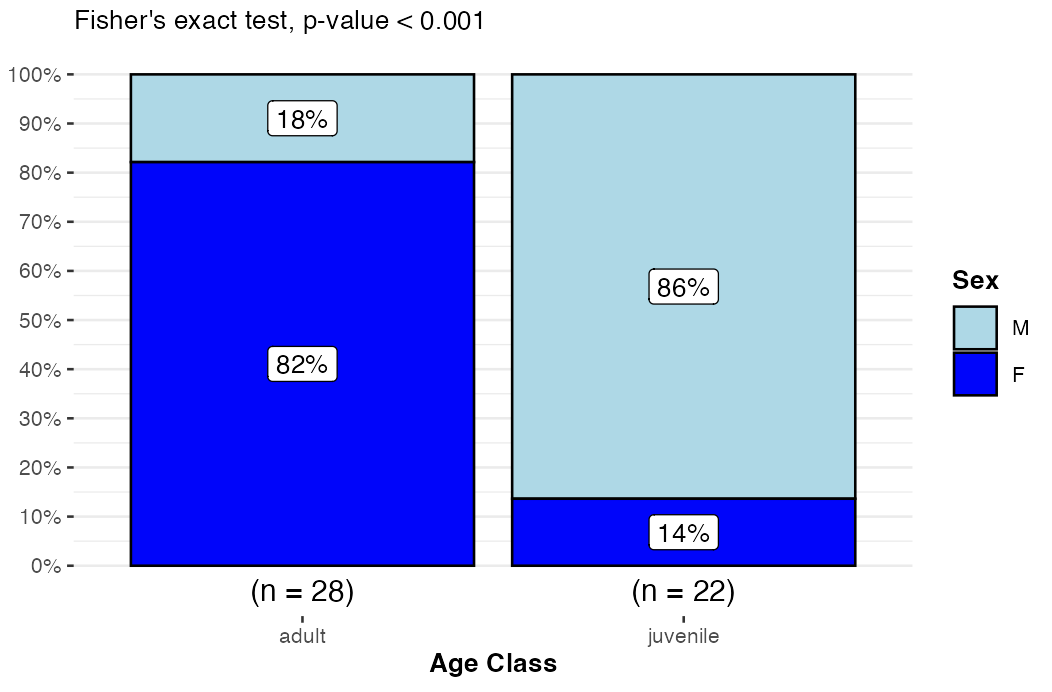
\includegraphics[width=4.75in,height=\textheight,keepaspectratio]{fisher_graph.png}

}

\caption{\label{fig-five}Proportion of sexes by age class, with adults
more frequently being female and juveniles more frequently being male.}

\end{figure}%

\textbf{Logistic Regression}

Data used for logistic regression analysis failed to meet assumptions.
Specifically, the data is non-normally distributed and has unequal
variance. As such, we were unable to conduct logistic regressions as
planned.

\textbf{Frequency Mapping}

As depicted in the graph, there are three main locations on which seals
haul out with shark bites: the north end, south end, and middle of the
colony (Figure 6).

\begin{figure}

\centering{

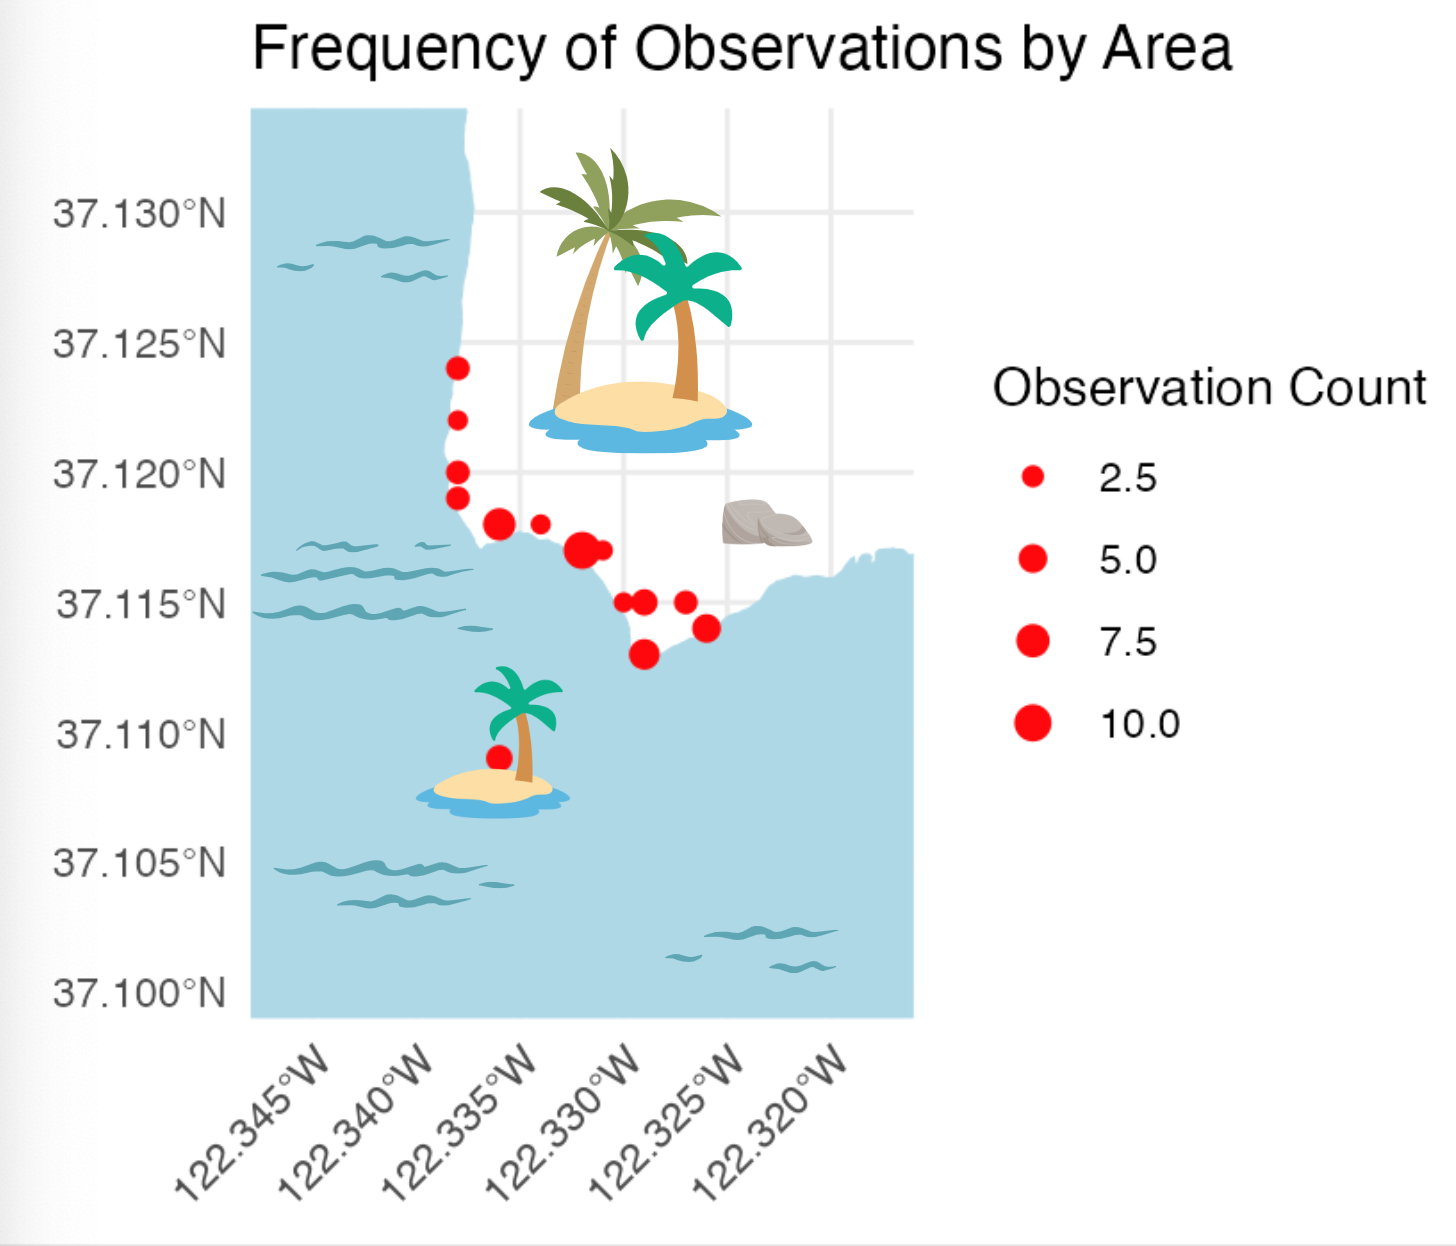
\includegraphics[width=3.64583in,height=\textheight,keepaspectratio]{map_graph.png}

}

\caption{\label{fig-six}Georeferenced frequencies of seal observations
per regionID area. Per EDA, most seals were found at either end of the
colony and the middle of the colony.}

\end{figure}%

\section{Discussion \& Conclusion}\label{sec-conc}

Our original research questions aimed at identifying trends in shark
bite survivorship. We found that survivorship differs significantly
against sex and age classes, with female adults and male juveniles
exhibiting bites most frequently. This result suggests that different
age classes and sexes exhibit different patterns in survivorship, and
perhaps predation, possibly due to their different body sizes and
foraging ecologies.

Unfortunately, analysis assumptions were not met for our logistic
regression analyses, so we were unable to explore quantitatively whether
or not age or sex predict shark bite location on the body. However,
exploratory data analysis suggests that female seals may have a
disproportionately high number of bites on their body (as opposed to
flippers or head or rear) compared to male and unidentified seals.

Finally, mapping efforts demonstrate that shark-bitten seals appear more
frequently on the main beach areas of the colony: North Point, South
Point, and Mid Bight. These locations align well with anecdotal reports
which suggest that seals aggregate more frequently in these large
beaches over inland gullies and vegetated areas.

Our results are limited by the survivorship bias that prevails in
on-shore sight-resight efforts. Current research being conducted in
collaborating labs seeks to characterize predator movement ecology to
better understand the trends observed here. Future work may also
consider the role of prey sex and age class in optimal foraging of
predators. Finally, ongoing research aims to describe aggregation
patterns of seals by microhabitat characteristics such as substrate
type. As stated at the beginning of this report, these research projects
serve the scientific knowledge base by contributing a fundamental
understanding of ecological dynamics across several ecosystems. This
work informs the conservation and regulation of key marine species and
environments during this era of extreme climate change.


\renewcommand\refname{References}
\bibliography{bibliography.bib}



\end{document}
